%======================================================================
\chapter{Liquid-Suspended CNT Experiments}
%======================================================================
\section{HCPBF Bandgap Overlap with CNT Excitation and Emission}
To successfully collect the CNT fluorescence when suspended within a HCPBF, the particle emission and excitation must be within the bandgap of the fiber. Taking the most commonly available HCPBFs, Table 4.1 shows the bandgap range and the central operating wavelengths for core-filled and fully D${}_2$O-filled fibers. In Fig.\ref{fig:cntoverlap}, the liquid-filled HCPBF bandgaps are overplayed with the excitation and emission spectrums of CNTs calculated in the previous section. From this overlay, it appears that 10 chiralities of CNTs fall within the bandgap of a fully-filled 1550nm HCPBF and one within the bandgap of  fully-filled 1060nm HCPBF. The potential CNT candidates and their characteristics are listed in Table \ref{cnt1550} along and their spectrum plotted within the 1550nm fully-filled bandgap in Fig.\ref{fig:cnt1550}.\\\\
\begin{tabularx}{\textwidth} { 
		| >{\centering\arraybackslash}X 
		| >{\centering\arraybackslash}X 
		| >{\centering\arraybackslash}X 
		| >{\centering\arraybackslash}X | }
	\hline
	HCPBF & Central Wavelength Air (nm) &  Central Wavelength D${}_2$O (nm) & Bandwidth (nm)\\
	\hline
	HC2000 & 2000 & 1144 & 250\\
	\hline
	HC1550 & 1550 & 887 & 500\\
	\hline
	HC1060 & 1060 & 606& 100\\
	\hline
	HC800B & 800 & 457 & 200\\
	\hline	
\end{tabularx}
\captionof{table}{ Thorlabs fiber bandgap shift. The ranges for HC1550 and HC800B are approximated from spectrum measurements and HC2000 and HC1060 are taken from NKT datasheets\cite{HC2000,HC1060}. \label{bgoverlap}}
\begin{figure}[htb!]
	\centering
	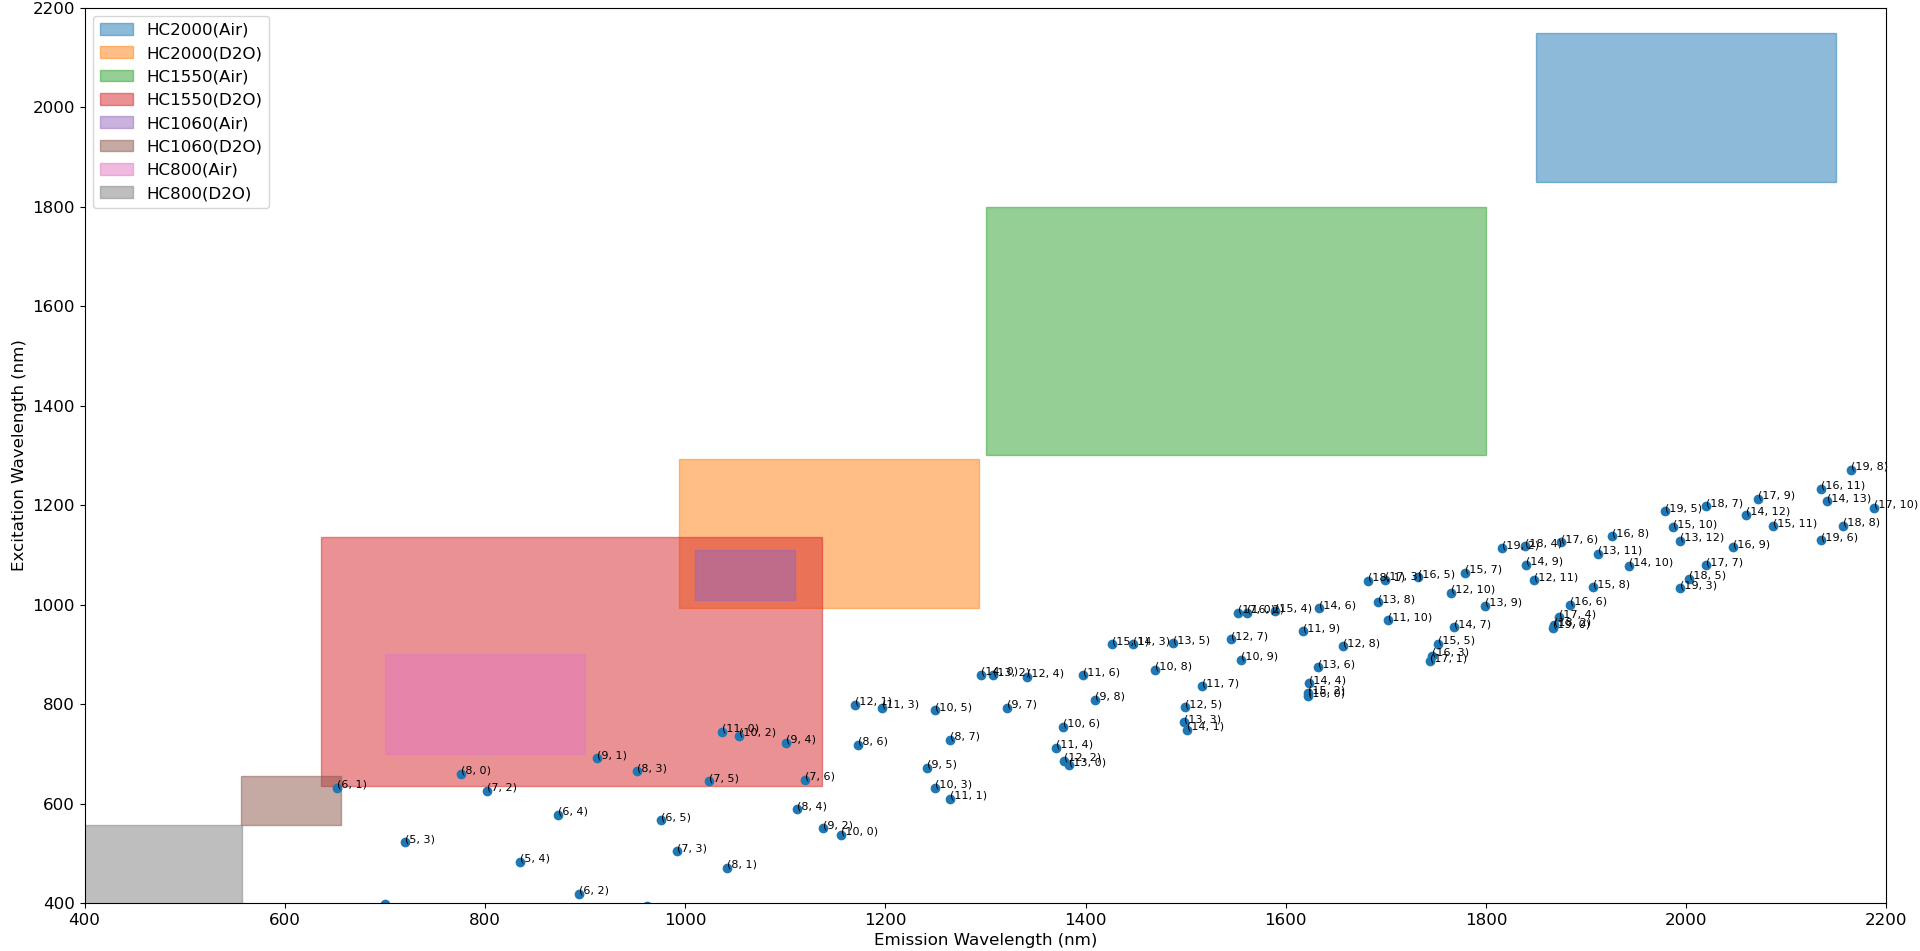
\includegraphics[width=\textwidth]{./Figures/CNTs/fibers_cnt.png}
	\caption{ Hollow-core fiber bandgap overlayed on CNT emission vs. excitation wavelengths }
	\label{fig:cntoverlap}
\end{figure}

\begin{figure}[htb!]
	
	\begin{minipage}{0.55\linewidth}
		\begin{tabularx}{\linewidth} { 
				| >{\centering\arraybackslash}X 
				| >{\centering\arraybackslash}X 
				| >{\centering\arraybackslash}X 
				| >{\centering\arraybackslash}X 
				| >{\centering\arraybackslash}X
				| >{\centering\arraybackslash}X
				| >{\centering\arraybackslash}X | }
			\hline
			$(n,m)$ & $dt$ (nm)	& $\Theta$ (deg) & 	$\lambda_{11}$ (nm)	 & $\lambda_{22}$ (nm)\\
			\hline
			(6, 1) & 0.52 & 0.13 & 652.62 & 631.79\\
			\hline
			(7, 2) & 0.65 & 0.21 & 802.05 & 625.92\\
			\hline
			(7, 5) & 0.83 & 0.43 & 1023.74 & 645.33\\
			\hline
			(7, 6)  & 0.89 & 27.46 & 1119.76 & 647.64\\
			\hline
			(8, 0) & 0.64 & 0 & 776.01 & 660.25\\
			\hline
			(8, 3) & 0.78 & 0.27 & 951.61 & 665.39\\
			\hline
			(9, 1) & 0.76 & 0.09 & 912.1 & 691.29\\
			\hline
			(9, 4)  & 0.92 & 0.31 & 1100.63 & 722.39\\
			\hline
			(10, 2) & 0.88 & 0.16 & 1053.43 & 736.68\\
			\hline
			(11, 0)  & 0.87 & 0 & 1036.93 & 744.57\\
			\hline
		\end{tabularx}
		\captionof{table}{ CNTs with emission and excitation transmittable through HC1550 filled with D${}_2$O. \label{cnt1550}}
	\end{minipage}
	\begin{minipage}{0.44\linewidth}
		\centering
		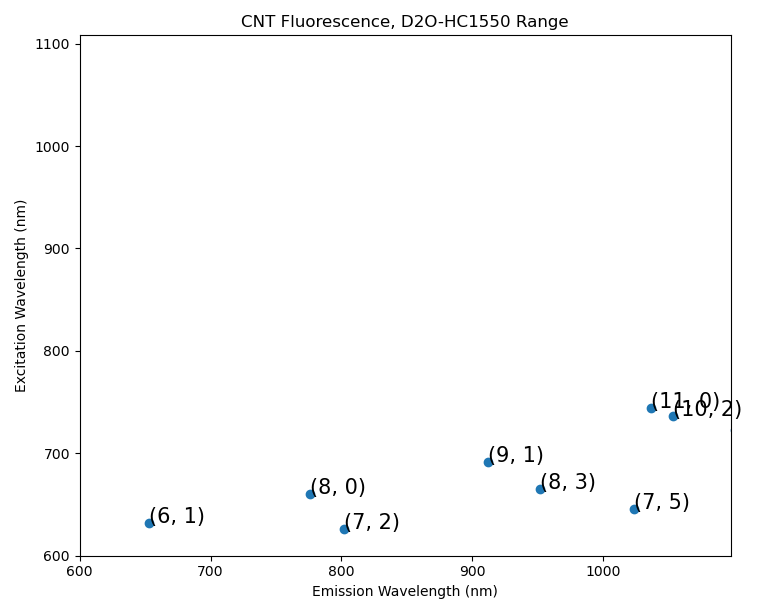
\includegraphics[width=9cm,height=7cm]{./Figures/CNTs/HC1550_range.png}
		\caption{ Excitation/Emssion spectrum of  CNTs falling within the D${}_2$O-filled 1550HCPBF bandgap.}
		\label{fig:cnt1550}
	\end{minipage}
\end{figure}

QuIN Lab at the University of Waterloo has developed a CNT isolation process using the surfactant sodium deoxycholate (DOC) in DI water, and are able to produce samples with (7, 6) and (7, 5) dominant samples. Thus far an experiential set-up for characterizing the CNT samples was completed, but use of the sample in HCPBF has not yet been completed. The sample information that has so far been collected is included.
\clearpage